\documentclass{article}


%preamble
%required
%\usepackage{Sweave} %Integrates R code with LaTeX for creating dynamic reports
\usepackage{natbib}%Provides citation and bibliography support
\usepackage{amsmath}%Enhances mathematical typesetting capabilities.
\usepackage{textcomp}%among other things, it allows degrees C to be added
\usepackage{float}%Helps with precise figure placement using the [H] option.
\usepackage[utf8]{inputenc} % allow funny letters in citations 
\usepackage[nottoc]{tocbibind} %should add Re fences to the table of contents?
\usepackage{amsmath} % making nice equations 
\usepackage{listings} % add in stan code
\usepackage{xcolor}
\usepackage{capt-of}%allows me to set a caption for code in appendix 
\usepackage[export]{adjustbox} % adding a box around a map
\usepackage{lineno}
\linenumbers

% recommended! Uncomment the below line and change the path for your computer!
% \SweaveOpts{prefix.string=/Users/Lizzie/Documents/git/teaching/demoSweave/Fig.s/demoFig, eps=FALSE} 
%put your Fig.s in one place! Also, note that here 'Fig.s' is the folder and 'demoFig' is what each 
% Fig. produced will be titled plus its number or label (e.g., demoFig-nqpbetter.pdf')
% make your captioning look better
\usepackage[small]{caption}

\usepackage{xr-hyper} %refer to Fig.s in another document
\usepackage{hyperref}

\setlength{\captionmargin}{30pt}
\setlength{\abovecaptionskip}{0pt}
\setlength{\belowcaptionskip}{10pt}

% optional: muck with spacing
\topmargin -1.5cm        
\oddsidemargin 0.5cm   
\evensidemargin 0.5cm  % same as odd side margin but for left-hand pages
\textwidth 15.59cm
\textheight 21.94cm 
% \renewcommand{\baselinestretch}{1.5} % 1.5 lines between lines
\parindent 0pt		  % sets leading space for paragraphs
% optional: cute, fancy headers
\usepackage{fancyhdr}
\pagestyle{fancy}
%\fancyhead[LO]{Frederik Baumgarten}
%\fancyhead[RO]{Research Proposal}
% more optionals! %

\usepackage{graphicx}
\graphicspath{{/Users/frederik/github/PlantDeterminism/figures/}} % specify the path to your figures directory




\begin{document}
	
	
	% Format for a letter in "Ecology Letters"
	\title{Invest now, get paid later? Growth strategies to cope with environmental stress and benefit from extended growing seasons in a future climate %(my favourite)
		
		%dlDec18: Alternate title ideas:
		%Growth determinism/determinacy/habits in plants/woody perennials/trees: Limits and opportunities of species to time growth activities in a future climate. 
		
		%Growth determinacy in temperate trees: investing at the right time to cope with environmental stress and benefit from extended growing seasons in a future climate.
	} 
	
	\date{\today}
	\author{Frederik Baumgarten\textsuperscript{1,2}, potentially with Yann Vitasse, EM Wolkovich, Sally and Rob)}
	\maketitle
	
	$^1$ Department of Forest and Conservation, Faculty of Forestry, University of British Columbia, 2424 Main Mall
	Vancouver, BC Canada V6T 1Z4. \\
	
	
	
	$^2$  Swiss Federal Institute for Forest, Snow and Landscape Research WSL, Zürcherstr. 111, Birmensdorf 8903, Switzerland\\ \\
	
	Corresponding Author: Frederik Baumgarten frederik.baumgarten@ubc.ca \\
	
	%Full word count: \\
	%Summary word count: \\
	%Introduction word count: \\
	%Materials and Methods word count: \\
	%Results and figure legends word count: \\
	%Discussion word count: \\
	
	
	\newpage
	
	\section*{Abstract} %150 words
	
	Although plants grow throughout their lifetime, the timing of growth activities within a growing season varies considerably across species. In the case of the primary meristem responsible for extension growth, most tree species in all biomes preform a considerable amount if not all of the tissue inside buds that will get deployed quickly after passing a state of rest/dormancy (determinate growth). This strategy is contrasted to various extend/degree by species which continue to generate new tissue during the current growing season (neoformed tissue, indeterminate growth). The implication of such growth habits has rarely been examined in the context of climate change, particularly given the increasing frequency of extreme weather events and extensions of the climatic growing season.  Here, we shed light on existing concepts of shoot extension phenology and debate which growth strategy may provide an evolutionary advantage. I propose that 1) determinate species may be more resistant and resilient to environmental stressors (e.g. drought) and 2) the higher the degree of indeterminacy in a species, the greater its capacity/potential to profit from extended growing seasons. Consequently, the question of how much carbon will be sequestered in a future climate might depend not only on abiotic factors like water availability, temperature extremes and the length of the growing season, but also on the degree of determinacy set by a species' intrinsic genetic programming. The accuracy of models predicting future carbon uptake by vegetation could be significantly improved by incorporating these traits which define a plant community's potential to respond to extended growing seasons in a specific region.
	\\
	
	\textbf{Keywords}: plant growth, tree phenology, shoot extension, indeterminate growers, carbon sequestration, growing season length, drought, genetic programming, phenotypic plasticity
	
	% Type of article: Letter
	
	\section*{Introduction}
	The further one travels from the equator towards the poles, the tighter plants are confined to a shrinking ‘time window of opportunity’ set by low temperatures (frost) and water restrictions (drought). While annual plant species accommodate their entire life cycle within this period, seasonal climates urge perennials to split their growing phases into annual chunks with periods of activity alternating with a period of rest (dormancy). This is referred to as intermittent or rhythmic (as opposed to continuous) growth.  
	
	 \citep{borchertClimaticPeriodicityPhenology1999, borchertComputeraidedEvaluationShootgrowth1976}
	\citet{boojhGrowthStrategyTrees1982}  
	\citep{borchertClimaticPeriodicityPhenology1999}
	\citep{rossiPatternXylemPhenology2016a}
	\cite{} 
	asdfasdfasdf
	\subsection*{The concept of determinism}
	A prerequisite of such plants inhabiting regions with distinct seasons is the ability to pre-form tissue as a future investment. Some species have their entire canopy build and packed in overwintering buds to be ‘ready to go’ when spring arrives, with no additional leaves and shoots being produced over the course of the growing season. This growth strategy is contrasted to various degree by species being able to form new tissue on top of preformed ones, sometimes stretching their continuous production until the end of the season. Although there is likely a wide spectrum of intermediate stages, species’ growth habits are commonly classified in a dichotomic way: determinate- or indeterminate growers.
	
	\subsection*{Aims}
	Most of our understanding of growth habits or growth determinacy in trees dates back to a period in the mid 1900s. The literature is sprinkled with different terms, concepts, and definitions spanning the fields of genomics, physiology and ecology across the animal and plant kingdom. However, and particularly for trees, the fundamental questions regarding the timing and duration of growth remain and are more pressing than ever: When and how much is growth and therefore carbon sequestration most impacted by climate extremes? Moreover, we must question the potentials and limits of trees to adapt - are they plastic enough to extend their growing period in a climate with prolonged seasons? Or are they bound to follow an internal program in which growth and development occurs within narrow temporal boundaries?
	
	In this review I aim to shed light on old concepts about the ability of plants to:
	a) preform tissue (i.e. structural growth) as a future investment that is ready to be deployed in spring with sustained growth thereafter (determinate strategy)
	b) maintain a somewhat constant growth activity by forming new tissue during the growing season (indeterminate strategy)
	and bridge the before mentioned research disciplines by scrutinizing these concepts across various scales: from the expression and regulation of specific genes and hormones that control growth-related processes to the large-scale consequences on ecosystems. 
	\\
	\subsection*{Definitions (in a box or as a schematic figure):}
	All plants add to their primary bodies as long as they live and can therefore be considered ‘indeterminate growers’ like mollusks, fish and reptiles (Ejsmond et al., 2010). However, plant physiologists use this term more specifically to address when extension growth occurs.\\
	Determination: The process of cells committing to a particular fate during their development. Specifically, the point at which a cell or a cohort of cells has been set to develop into a specific tissue or organ.\\
	Determinism: The idea that a plant’s development and characteristics are defined by its genetic program shaped by its environment. \\
	Determinacy: The characteristic of a plant to either stop growing after reaching a certain size or having produced a certain amount of flowers/fruits or to keep growing throughout its lifetime. E.g. two varieties of tomato plants that either stop growing with a fixed amount of fruits or continue to grow and produce fruits as long as conditions allow it. \\
	Growth habit: The genetic tendency of a plant to form a characteristic habitus (shape, height, form) with a particular branching and growth pattern. 
	determinate growth: a growth pattern characterized to stop at a predefined size. Commonly, the apical bud culminates in an inflorescence, halting the production of any additional leaves or buds. In trees this terms specifies the short duration of extension growth in spring with no further activity of the apical meristem.\\
	sustained growth:\\
	indeterminate growth: a growth pattern characterized by continuous growth (leaves, buds or flowers) throughout their life or as long as condition remain favourable. This is possible because the apical meristems always remain vegetative and flowers are restricted to lateral meristems. In trees this refers to the continuous shoot elongation throughout the growing season.\\
	Neogrowth: Growth that occurs on top of preformed tissue due to the more or less continuous activity of the shoot apical meristem. Several forms occur depending on whether growth occurs continuously or in bursts.\\
	Perpetual/Continuous/free growth: the constant production of new tissue without interruptions of bud stages.\\
	Polycyclic growth: Growth occurs in bursts after the initiation of leaf primordia inside buds.  \\
	Second flush: Growth form of species in which one additional cohort of buds is build and deployed during the current growing season. In the German literature this is often termed ‘Johannitrieb’ since the flush often occurs around the summer solstice. Also ‘lammas growth’ is a common term for an additional flush (lammas = loaf mass; old English for the holy communion typically to celebrate the first harvest).\\
	
	\subsection*{How is primary growth controlled?}
	\subsection*{Across scales: from cellular to organ to whole plant level}
	the cellular level with omnipotent cells differentiating into specialized cells, organ levels to whole plant level (organism), annual plants dying after the season once they have flowered and produced fruits. programmed cell death as another example.
	Merophytes: Group of cells that are derived from one meristem. Its the basic repeatable unit or structure of a plant\\
	Organ level: leaves, flowers and fruits grow determinately; shoot, cambium and roots grow indeterminately\\
	Phytomers: The LEGO-Piece from which plants are build. The basic unit of the physical structure of a plant. Typically it consists of a leaf, a node, an internode and a bud. Phytomers contribute to the segmented or modular structure of plant growth. \\
	Plant level:\\
	Age effects ontogeny: every plant that starts from a seat grows always in indeterminant way then with age increasingly become more conservative and determinant\\
	
	a common definition of determinate growth is that organisms stop growing when maturity is reached or shortly afterwards. whereas indeterminate organisms continue to grow over their lifetime.\\
	perennial plant add to their primary bodies as long as they live. \\
	indeterminate growth in perennials means "the iterative production of determinate units"\\
	
	
	\subsection*{Internal control mechanisms of growth}
	A. Genes and molecular pathways\\
	- Role of specific genes in determining shoot growth patterns\\
	- Molecular pathways involved in controlling shoot growth \\
	
	B. Hormonal regulation \\
	- Apical dominance and its influence on shoot growth\\
	- Role of auxin and other hormones in determining shoot growth patterns\\
	- Physiological aspects of hormonal control in shoot growth determinism\\
	
	
	Allocation problems: imbalances of shoot and root growth\\
	In some cases shoot growth might come to a halt because of the demand of water cannot be met. Since above and belowground meristem experience large differences in temperature, the higher growth rate of shoots may soon result in a imbalanced root-shoot-ratio that can only be overcome by sustaining growth of the apical meristems until root growth has caught up to reach the supply capacity. High vapour pressure deficits and the resulting water transpiration or a drying soil might have the same effect. This could also explain polycyclic flushing patterns as a result of lower growth rates in roots.\\
	This hypothesis is also supported by experimental data. Artificial reduction of leaf area caused terminal buds to keep growing until leaf area was re-established.
	Is there a different strategy in allocation to roots or shoots tissues depending or associated with a species degree of determinism of a species. In other words is the imbalance of root to shoot ratios caused by environmental differences or by an internal program regardless of environmental conditions. \\
	
	
	\subsection*{External control mechanisms of growth}
	- Influence of temperature, water availability, vapor pressure deficit and nutrient availability on shoot growth patterns\\
	
	\subsection*{Sink source relationships}
	temporal separation of growth investments (sinc activity) from their returns when deployed (source activity). \\
	
	\subsection*{Growth Transitions}
	Switch from growth acquisition to maturation and reproduction as well as preparing for winter and storage\\
	
	
	\subsection*{External control mechanisms of growth}
	- Influence of temperature, water availability, vapor pressure deficit and nutrient availability on shoot growth patterns\\
	
	\subsection*{Evolutionary perspectives}
	Patterns of shoot elongation determines the timing of a fully developed canopy\\
	The reason of differences in determinism or shoot elongation patterns is to launch the photosynthesis apparatus/capacity at once (determinate strategy) with an inevitable decline as leaves age or to spread resources more steadily across the growing season increasing the canopy area or replacing losses (indeterminate strategy). So when is the best time to display the leaves? And what are the trade-offs involved? Flushing early in spring might extend the growing season benefiting from early accessible resources (water, nutrients, light). However, at this time of the year spring frost damages represent a risk and are particular costly if most of the leaf area is invested at once. This is probably why determinate growing species are often among the latest flushing species. Indeterminate species can quickly compensate for losses while benefiting in some favourable years. \\
	
	Herbivory: A continuous production of leaves compensates for herbivory losses. Moreover, timing leaf emergence in bursts can reduce the population of leaf consuming insects.
	cost of indeterminate growth: they keep producing until the last cohort of leaves are hit by frost with potential losses in nutrients. \\
	Constant ideal conditions in the tropics only a few species perform constant growth in this ideal growing conditions most of the trees still accept it bursts of growth this might be an adaptation to parasites and heavy voice to reduce available food sources in some years to reduce population sizes of antagonists is there a latitudinal gradient with species exhibiting a more deterministic strategy the same trends could also be seen along a continentality gradient. With ecosystems on the oceanic range consisting mostly species with indeterminate strategies and on the continental extreme ecosystems harbouring mostly species with a determinate strategy\\
	
	Phylogenetic questions: Is indeterminate growth the original/older strategy?\\
	
	\subsection*{The role of determinism with climate change}
	Increased environmental stress\\
	Stressors such as drought and frost can disrupt the phenological cycle of a tree opening the questions which growth strategy is more plastic. can a species compensates for some stress-induced losses later in the season?\\
	
	Growing season extended\\
	what happens if the growing season extends due to climate warming? which growth strategy allows to profit most from this opening window of opportunity? This might mix competition among co-occurring species and might change species and community assemblages in the future with more indeterminate species most likely gaining ground because they might be plastic enough to fill this gap. \\
	carbon sequestration? Productivity and longevity. which strategy allow for more carbon uptake in the long run or at least integrated over few years because of different allocations within one growing season into buds, reserves, roots etc.
	which strategy leads to taller or bigger structures that are durable and live longer? this will decide over the residence time of carbon in an ecosystem.
	\\
	\pagebreak

	
	\begin{figure}
		\centering
		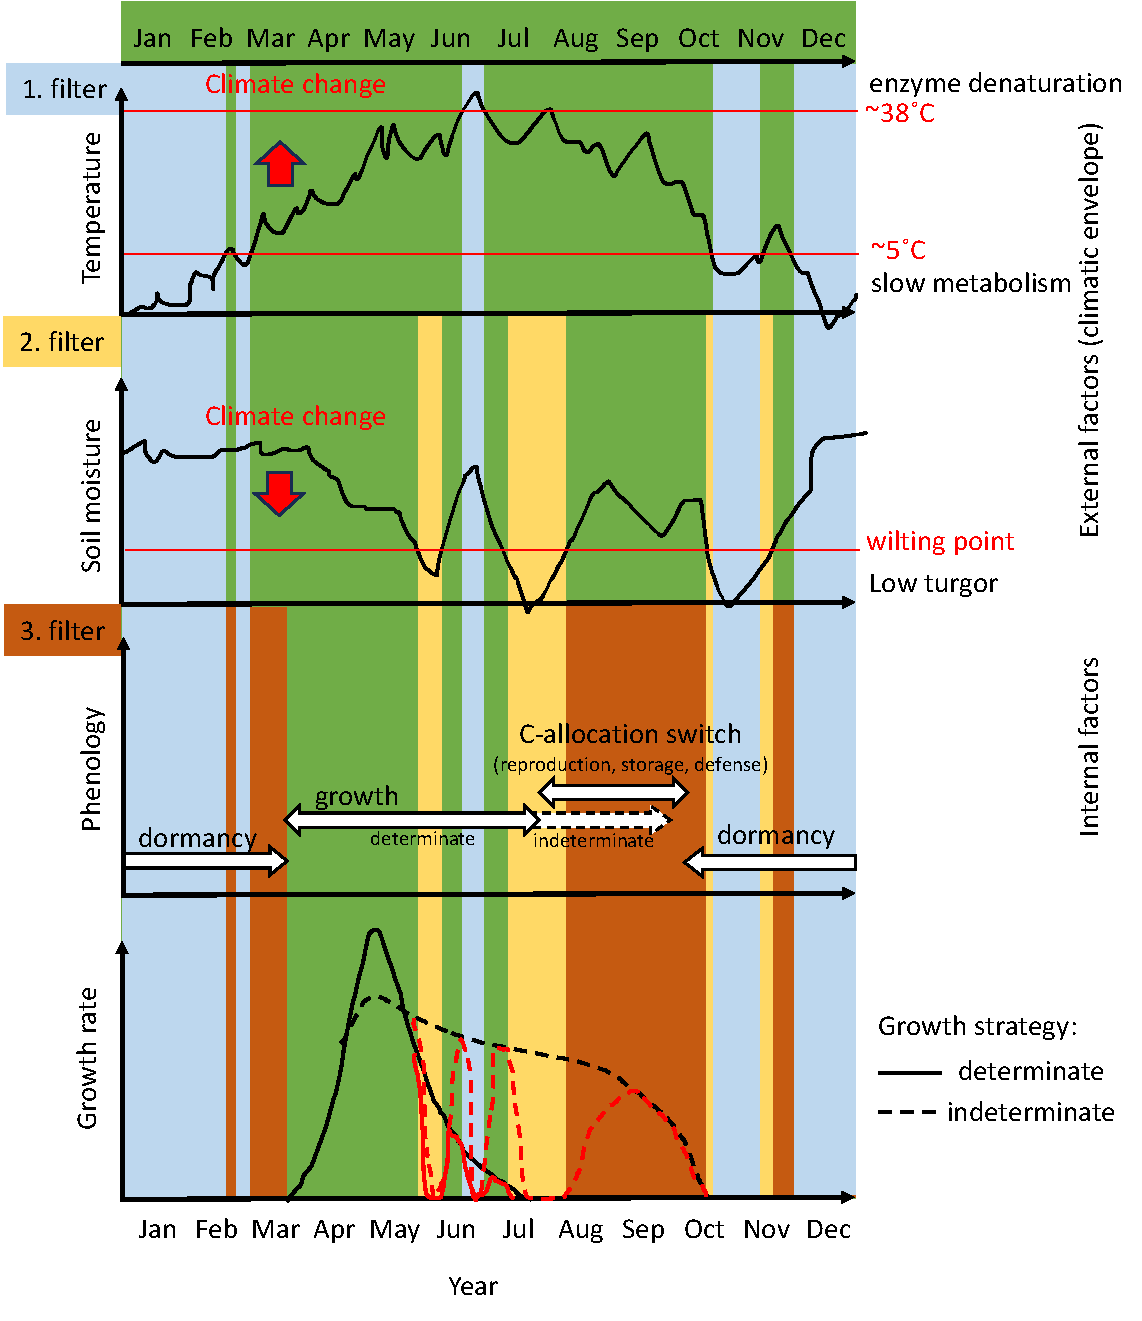
\includegraphics[width=0.9\textwidth]{Fig_1_V2.pdf} 
		\caption{Schematic overview of the discrepancy between the potential growing season and the effectively realized vegetative growth. Environmental factors like temperature and soil moisture, exceeding growth-promoting thresholds can be seen as filters that narrow the window of opportunity available for vegetative growth. The species-specific life history cycle (phenology) can further impose another filter by imposing a dormancy cycle and/or prioritizing developmental processes other than structural growth (e.g. flowering, fruit maturation and storage). }
		\label{fig:your-figure-label-xxx}
	\end{figure}
	
		\pagebreak
		
	\begin{figure}
		\centering
		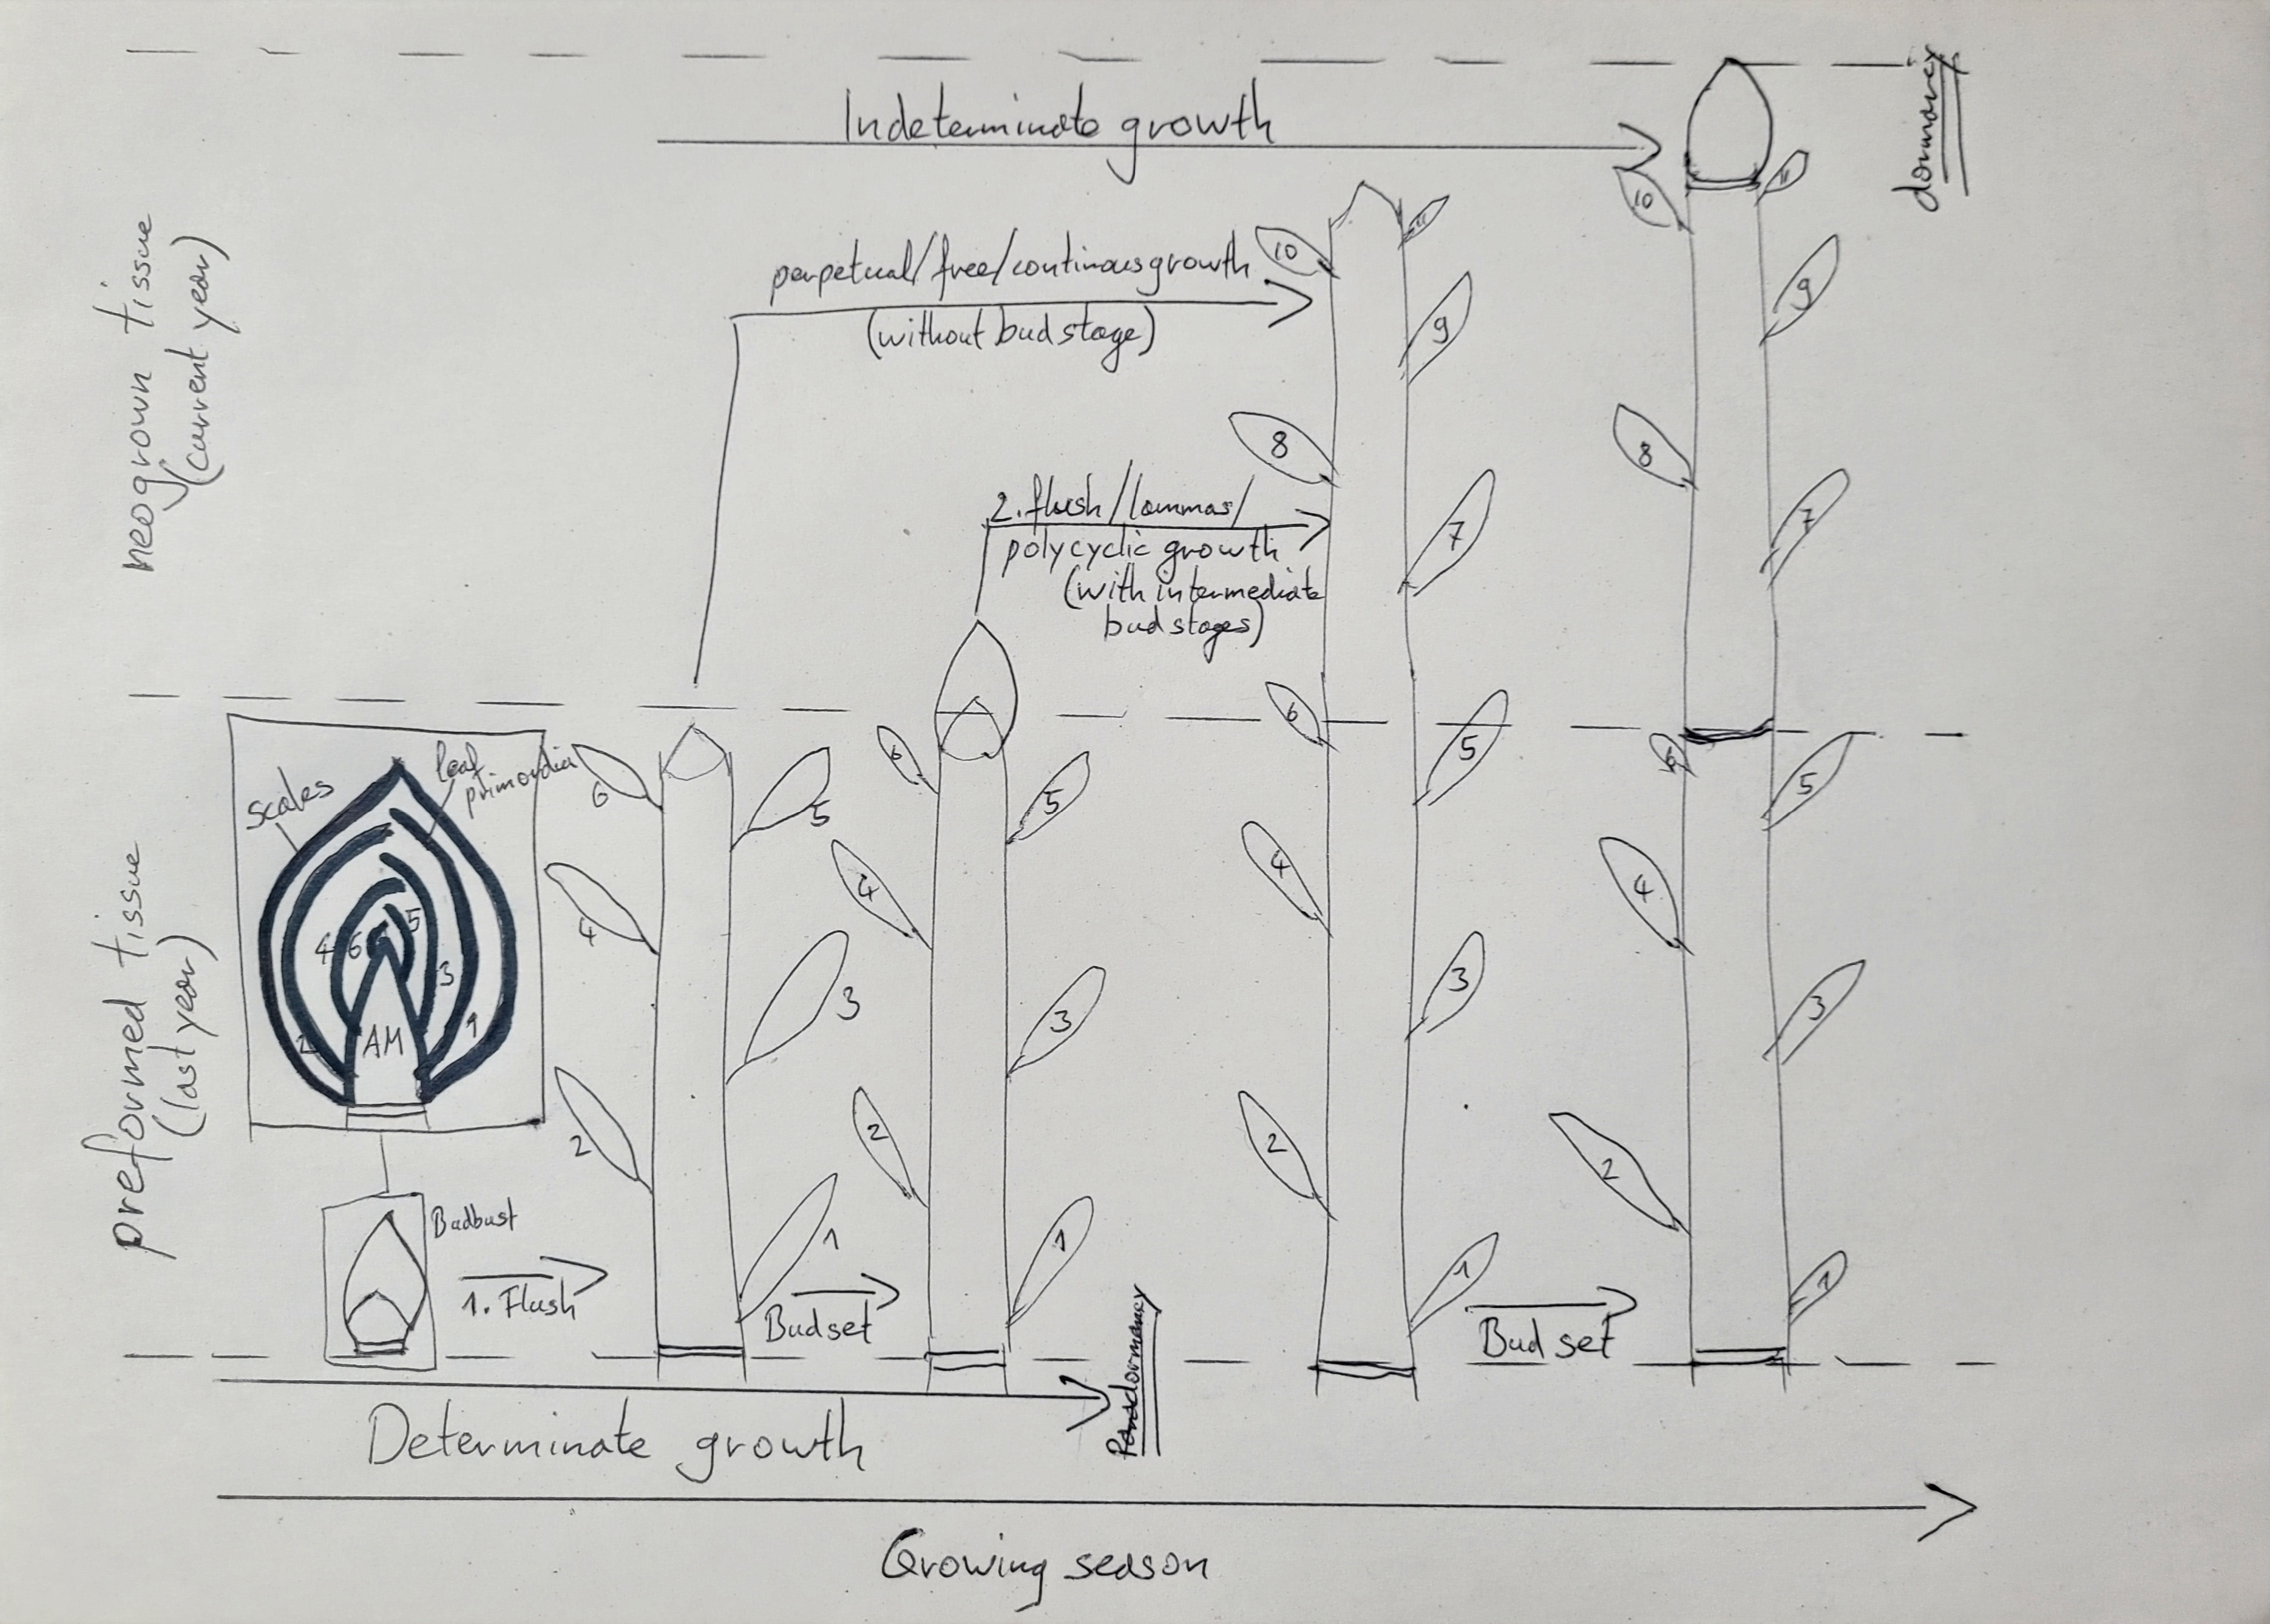
\includegraphics[width=1.1\textwidth]{Fig_2.jpg} 
		\caption{Determinate and indeterminate growth within one growing season. Commonly all tree species deploy buds during their first spring flush from prebuild and overwintering leaf primordia (A-B). Determinate growing species set bud that are under hormonal suppression (paradormancy) to sustain any further activity of the shoot apical meristem (C). Indeterminate growing species continue to produce new tissue directly (D) or through one or several intermediate bud stage(s) (E). Finally all species set their bud and enter endodormancy}
		\label{fig:your-figure-label-xxx}
	\end{figure}
	
		\begin{figure}
		\centering
		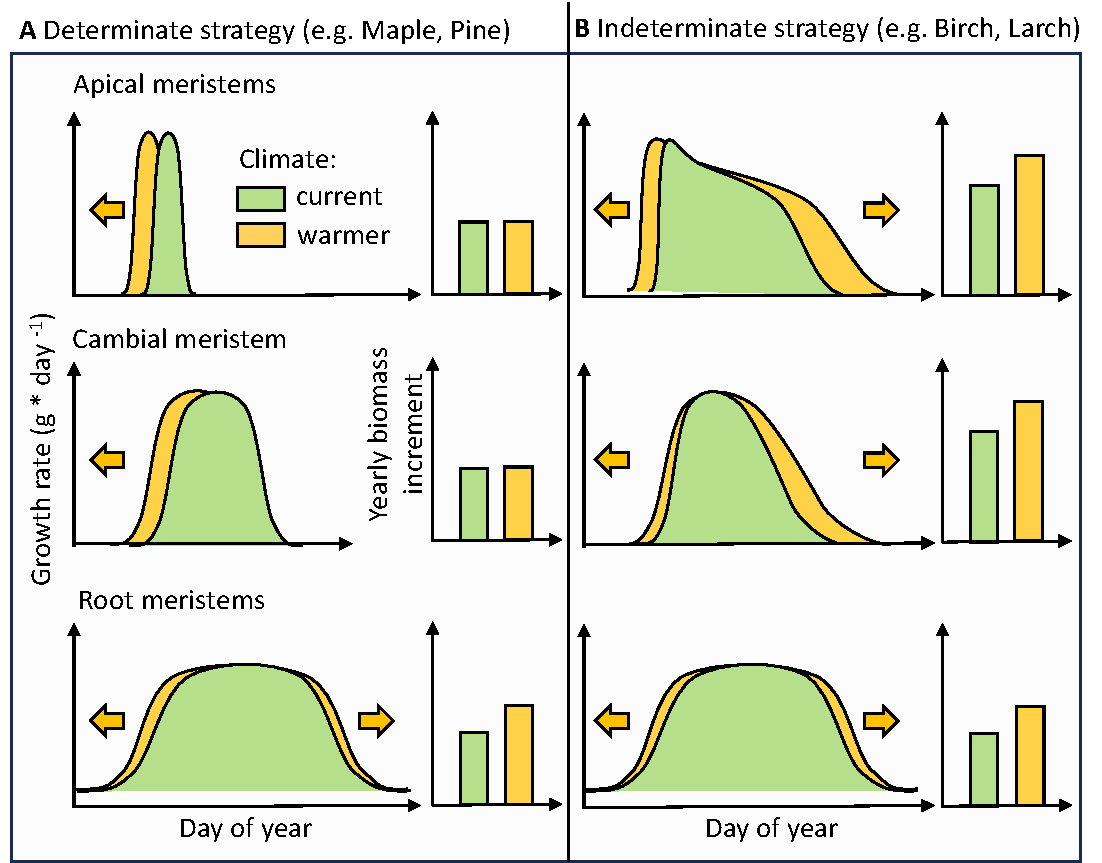
\includegraphics[width=0.9\textwidth]{Fig_3_V2.pdf} 
		\caption{Hypothesized predictions of growth rates for the three major meristems (apical, cambium and root) classes of trees under current and warmer climates following an extreme determinate (A) and indeterminate (B) growth strategy. The area under the curve is summarized as yearly biomass increment in the respective bar-plot. Arrows indicate the shift of growth phenology under warmer climate conditions. Root meristems appear to be purely temperature-opportunistic for both strategies, even growing during warm winter spells. The indicated genera were observed to showcase the illustrated trends. The responses of these two contrasting growth strategy might apply not only to different tree species but also within a population (e.g. along environmental gradients) and even within an individuum as it transitions from the junvenile to the adult stage (ontogeny).}
		\label{fig:your-figure-label-xxx}
	\end{figure}
	
	Figure \ref{fig:your-figure-label-xxx} shows an example figure.
	
		\newpage
	
	\bibliography{Growth_determination}
	\bibliographystyle{apalike}
	
	
	
\end{document}



